% !TeX encoding = utf8
% !TeX program = xelatex
% !BIB program = bibtex
%
% Configuration options:
% english - Use for English language theses
% german - Use for German language theses
% ba - Use for Bachelor theses
% ma - Use for Master theses
\documentclass[german,ma]{tudo-sse-thesis}

% Add the packages necessary
\usepackage[math]{blindtext}

% Provide your title
\title{Thesis Title}

% Provide your name
\author{Firstname Lastname}

% Provide examiner names. First examiner has a reasonable default and only needs to changed if the default does not fit.
% \firstexaminer{JProf.\ Dr.-Ing.\ Ben Hermann} % Default value
\secondexaminer{Prof.\ Dr.\ Zweiter Gutachter}

\begin{document}

\maketitle

\pagenumbering{roman}

% Only add for english documents
\begin{abstract}
  This is an Abstract. \blindtext
\end{abstract}

% This needs to be in German or English documents
\begin{abstract-ger}
  Dies ist eine Zusammenfassung.  ßäöü \blindtext
\end{abstract-ger}

\tableofcontents
\cleardoublepage

\pagenumbering{arabic}

% Add your content here
\chapter{Introduction}
\section{Motivation and Background}
Example reference~\cite{AggarwalV88}.
\section{Thesis Structure}
\chapter{Example Chapter}
\label{ch:sample-chapter}



% Bibliography
\bibliographystyle{ACM-Reference-Format}
\bibliography{bibliography/references}
\addcontentsline{toc}{chapter}{\bibname}

\cleardoublepage
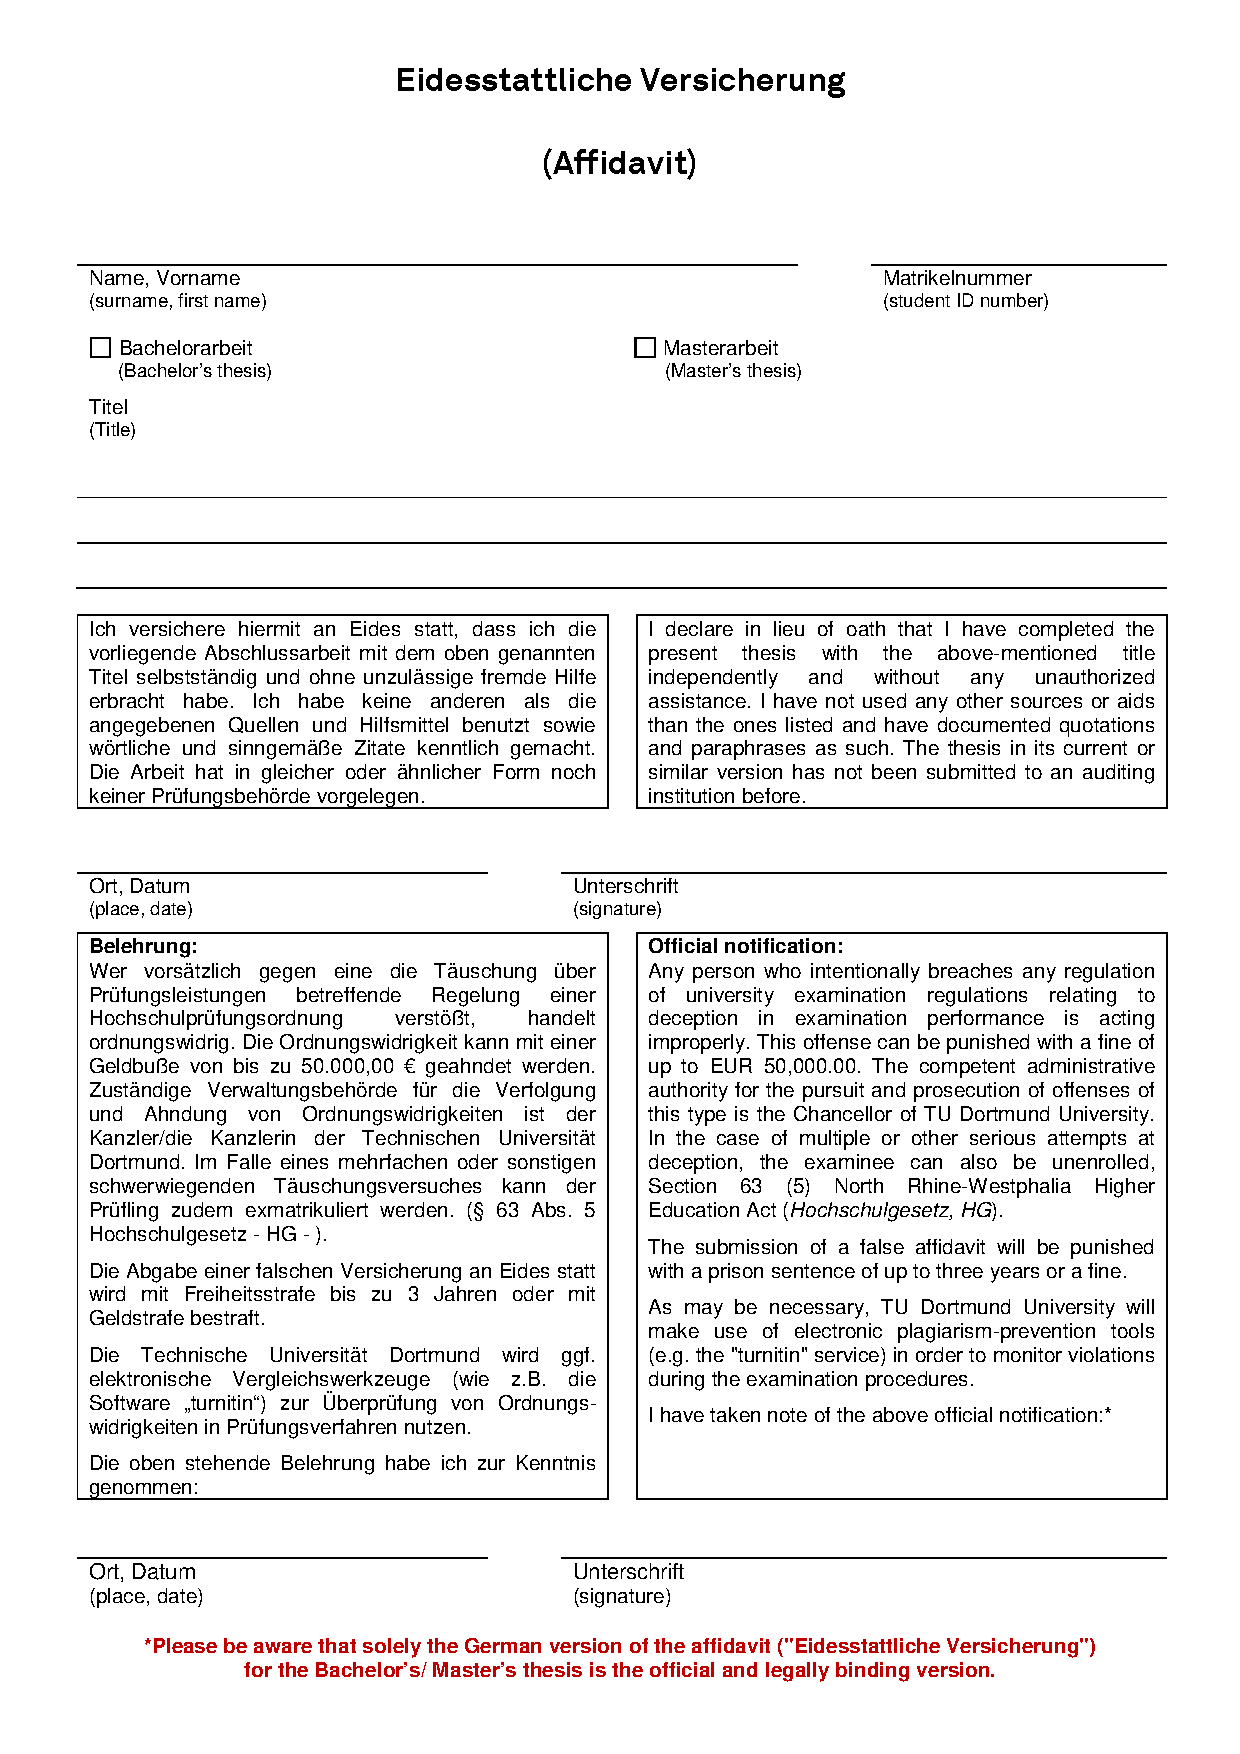
\includepdf[pages=-]{Eidesstattliche_Versicherung}

\end{document}
